\documentclass[11pt,a4paper,ngerman]{report}
\usepackage{babel}
\usepackage{float}
\usepackage[utf8]{inputenc}
\usepackage[T1]{fontenc}
\usepackage{amsmath}
\usepackage{amssymb}
\usepackage{graphicx}
\usepackage{subfig}
\usepackage{csquotes}
\usepackage[backend=bibtex,natbib=true,style=alphabetic]{biblatex}
\addbibresource{Quellen.bib}

\date{\today}
\title{Belegarbeit zur Quellenkodierungsmethode \textbf{"Run-Length Encoding"} im Modul "statistische Nachrichtentheorie"}
\author{Von: Monique Golnik (563075) \\Dozent: Prof. Dr. Christoph Lange}






\begin{document}

	\maketitle
	\tableofcontents


	
	\chapter{Einleitung}
	In der heutigen Zeit ist es wichtiger den je sich mit der Komprimierung von Daten auseinander zu setzen. Auch wenn die Speicherkapazität einem das Gefühl der Grenzenlosigkeit vermittelt, entspricht das nicht der Realität - Kompressionsverfahren sind nicht mehr wegzudenken und gewinnen stetig an Bedeutung.
	
	
	Gegenstand dieser Belegarbeit ist die nähere Betrachtung einer Quellcodierung, wobei  \textbf{Run-Length Encoding} im Fokus steht.
	
	
	Ziel ist es, dass ein Verständnis der Funktionsweise dieses Verfahrens und dessen Grenzen vermittelt werden.
    
    
	Zunächst werden in Kapitel 2 grundlegende Begrifflichkeiten näher erläutert und es wird in die Thematik der Quellenkodierung und Datenkompression eingeführt. In Kapitel 3 wird das Verfahren Run-Length Encoding definiert, Vor- und Nachteile benannt sowie Anwendungsbeispiele dargestellt, um den Einsatz zu verdeutlichen



	\chapter{Quellenkodierung und Datenkompression}
	
		Bei der Quellkodierung ist es das Ziel, dass die Symbolentropie erhöht und so die Redundanz reduziert wird. Sie ist eine eineindeutige Darstellung der Quelleninformation in einer realisierbaren und möglichst redundanzfreien beziehungsweise -armen Form.
		
		Die Aufgabe der Quellenkodierung ist die Kodierung eines Datensatzes, der von einer Informationsquelle abgegeben wurde, in einen Binärcode mit möglichst kleiner Stellenzahl. \cite[Seite 47 ff.]{Lange2021}
	     
	    \enquote{Bei der Datenkompression werden Dateien in eine alternative Darstellung überführt, die effizienter ist als die ursprüngliche. Ziel dieser Codierung ist es, sowohl den benötigten Speicherplatz als auch die Übertragungszeit zu verringern.} \cite{IONOS} 
	
		Durch zwei unterschiedliche Ansätze, lässt sich so ein Codiergewinn erreichen:
	
		\begin{itemize}
		\item \textbf{Redundanz-Kompression}: 
		Auf der Grundlage einer Redundanzreduktion lassen sich Daten nach der Kompression verlustfrei wieder dekomprimieren - eine solche Kompression ist nur möglich, wenn ein Datensatz sich wiederholende Zeichen beinhaltet
		
		\item \textbf{Irrelevanz-Kompression}:
		Bei diesem Ansatz werden irrelevante Informationen entfernt, um einen Datensatz zu komprimieren. Jedoch lässt sich dadurch der Datensatz nicht Bit-genau wiederhergestellten und ist somit verlustbehaftet
		\end{itemize}
	
	
		Im Folgenden wird der Blick auf die verlustfreie Kompressionsmethode \textbf{Run-Length Encoding} gerichtet und näher erläutert.
	
	
	\chapter{Run-Length Encoding}	
  		\section{Redundanz-Kompression durch \\ Run-Length Encoding}
  		  Die Lauflängencodierung \footnote{(Run-Length Encoding (RLE), Run-Length Coding (RLC), Lauflängencodierung = Synonyme} beschreibt eine verlustfreie Kompression, die sinnvoll angewandt werden kann, wenn der Datensatz Sequenzen mit sich mehrfach wiederholenden Zeichen enthält.
  		  
  		  
  		  Die RLE ist den sogenannten \textbf{Phrasencodern} zugeordnet, wie in Abbildung \ref{MMK} dargestellt.
  		  
  		  \begin{figure} [H]
  		  	\begin{center}
  		  		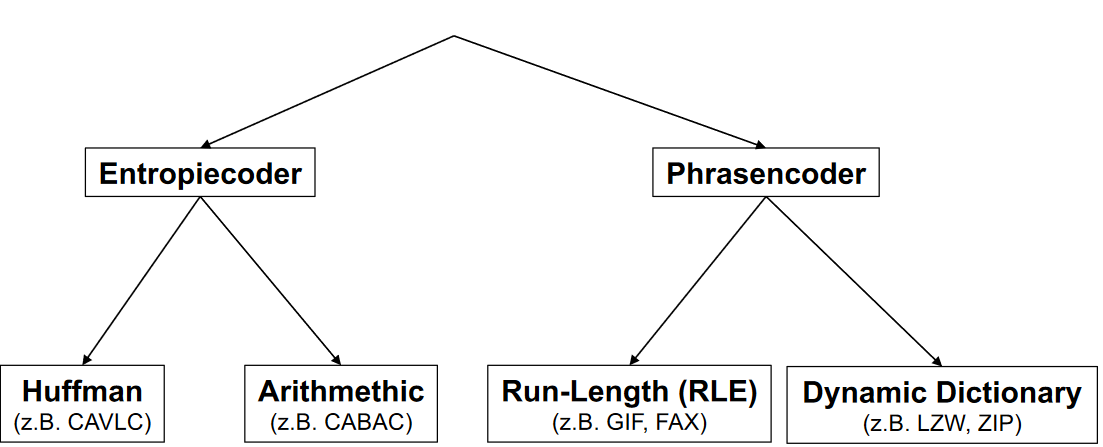
\includegraphics[width=0.75\textwidth]{MMK_RLE.png}
  		  		\caption{Klassifikation von verlustlosen Kompressionsmethoden}
  		  		\cite[Seite 8]{MMK}
  		  		\label{MMK}
  		  	\end{center}
  		  \end{figure}
  		  
  		  
  		  Bei dieser Art der Codierung wird eine Folge von gleichen Zeichen, Buchstaben oder Zahlen durch ein Symbol und die Angabe über die Häufigkeit der gleichen Symbole substituiert. Die Abfolge von identischen Zeichen und der Länge der jeweiligen Sequenz, die in einem sogenannten Run Counter gespeichert wird, wird als \textbf{Run} bezeichnet. Aufeinanderfolgende Vorkommen eines Datensatze $d = Run$. Anzahl der Wiederholungen $n$ von $d = RunLength$ (Lauflänge) Diese Form der Kompression eignet sich sehr gut um Redundanzen in Grafiken und Bilddateien mit wenigen Farben zu beseitigen.
  	  
  		  Ist die zu komprimierende Grafik sehr detailreich, besitzt also sehr viele Farben oder Kontraste, ist die Lauflängencodierung nicht mehr geeignet,  da so nur sehr selten gleiche Zeichen in einer Sequenz aufeinander folgen.\cite{ITWissen.info} Auch für Texte eignet sich diese Methode eher nicht, da hier zwar Farben eine untergeordnete Rolle spielen, jedoch die aufeinander folgenden Buchstaben sehr selten gleich sind und so einzelne Zeichen nicht effizient zusammengefasst werden können.\cite[Seite 61]{Lange2021}
  		  
  		  Bei der Kompression werden identische Zeichen so lange eingelesen, bis sich einer ändert - Zeichen und Anzahl die gleich sind, werden festgehalten. Bei der Dekompression wird der festgehaltene Wert ausgelesen und die dem entsprechende Anzahl an Bits ausgegeben.\cite{ITWissen.info}
  		  
  		  Sendet die Quellen neben Buchstaben auch Ziffern, so muss das Verfahren um Sonderzeichen erweitert werden, so dass die resultierende Angabe weiterhin eindeutig als Lauflänge gekennzeichnet ist. \cite[Seite 62]{Lange2021} Ein Beispiel zur Verdeutlichung findet sich in Abbildung \ref{Lange}.
  		  
  		   \begin{figure} [H]
  		  	\begin{center}
  		  		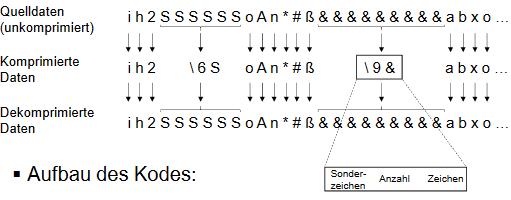
\includegraphics[width=0.75\textwidth]{alpha_ziffer.png}
  		  		\caption{Beispiel Verfahrenserweiterung}
  		  		\cite[Seite 62]{Lange2021}
  		  		\label{Lange}
  		  	\end{center}
  		  \end{figure}
  		  
  		  Der Kompressionsgrad des Run-Length Encodings hängt stark von der Charakteristik der Quelldaten ab. \cite[Seite 62]{Lange2021}
  		 
  		 
  		 
	
		\section{Vor- und Nachteile gegenüber anderen Verfahren}
		\textbf{Vorteile:}
		Das RLE-Verfahren zeichnet sich durch seine Geschwindigkeit und Einfachheit aus. Zudem zeichnet es sich durch eine signifikante Datenkompression aus, wie im Kapitel \textbf{Einsatz \& Anwendungsbeispiele} verdeutlicht wird.
		\\
		\textbf{Nachteile:}
		Auch wenn RLE signifikante Vorteile bietet, ist es aber zur Kompression komplexer Farbbilder ungeeignet- auch wenn das Verfahren weiterentwickelt wurde und dadurch die Zunahme des Datenvolumens bei Reihen ohne Wiederholungen kein Problem mehr darstellt, so sind die Kompressionsraten bei solchen Bildern doch denkbar schlecht. Der sinnvolle Einsatz von RLE beschränkt sich daher auf bestimmte Grafiktypen.\cite{Koeck2006}	Bei sehr kleinen Zeichenfolgen kann es passierten, dass sich die Daten sogar vergrößern, wie beispielsweise bei einem Schabrettmuster. Daher muss vorher eine Mindestanzahl von Werten die zusammengefügt werden gesetzt werden.
		
		
		
		
		
		\section{Einsatz \& Anwendungsbeispiele}
		Die Lauflängencodierung findet Anwendung bei verschiedenen Grafikdateiformaten, wie beispielsweise dem TIFF\footnote{TIFF = Tagged Image File Format}, dem TGA- und dem Bitmap- Dateiformat.In diesem Kapitel werden  Beispiele aus unterschiedlichen Bereichen dargestellt, um zu verdeutlichen, wo sich die Lauflängencodierung eignet und wie sie angewandt wird.
	
		\textbf{1. Einsatz in der Computergrafik}
		\\
		In diesem Bereich wird das RLE- Verfahren bei speicherintensiven Rastergrafiken angewendet und ist besonders effizient, wenn es sich um Grafiken mit wenigen aber großflächigen Farben handelt. Das Verfahren kann dabei sogar noch optimiert werden, in dem eine Wegoptimierung durch die Wahl des effektivsten Laufweges anhand eines Algorithmus vorgenommen wird.  Dieser Laufweg könnte beispielsweise zeilen-sequenziell, im Zick-Zack oder mäanderförmig\footnote{Mäander = Bezeichnung einer Flussschlinge in einer Abfolge weiterer Flussschlingen } siehe Abbildung \ref{mäander} sein.

		
		
		 \begin{figure} [H]
			\begin{center}
				\includegraphics[width=0.25\textwidth]{Mäander.png}
				\caption{Wegoptimierung: Mäanderförmig}
				\cite{kocerheiztech}
				\label{mäander}
			\end{center}
		\end{figure}
		
	  \textbf{Grafik mit 48 Bytes:} Die Lauflängencodierung lässt sich auf sogenannte Rastergrafiken\footnote{Rastergrafik = Pixelgrafik} übertragen, in dem die RGB-Werte genutzt werden.
	  
			\begin{itemize}
				\item \textbf{zwei Beispielabfolgen}: siehe unter RLE-Code (rechts) in der Grafik \ref{Effizienz}
				
				\item \textbf{RGB-Farbwerte:} Diese stellen die jeweiligen Farben  dar 
				\subitem Sind viele gleichfarbige Pixel (hier als Kästchen dargestellt) aufeinander folgend, können diese gut zusammengefasst werden, in dem die Anzahl vor dem Farbwert übertragen wird.
				
				
				
				
				\begin{figure} [H]
				\begin{center}
						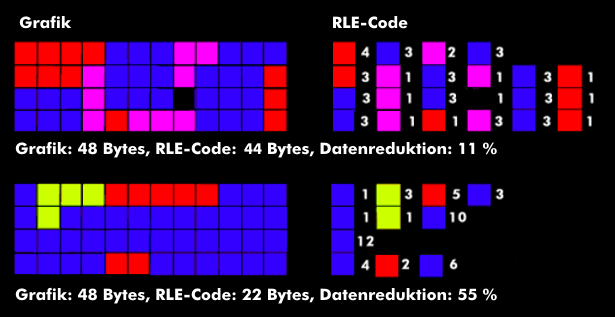
\includegraphics[width=0.75\textwidth]{g_h_Effizienz.png}
						\caption{Beispiel mit geringer und höherer Effizienz}
						\cite{ITWissen.info}
						\label{Effizienz}
					\end{center}
				\end{figure}
				
				\subitem In der Grafik \ref{Effizienz} wird auch schnell deutlich, dass ein sehr detailreiches Bild ungeeignet für die RLE-Codierung ist, da kaum gleichfarbige Pixel aufeinander folgen. Die Datenreduktion beträgt im oberen Grafikbeispiel gerade einmal 11\%. In der unteren, in der sich sehr viele nebeneinander liegende blaue Pixel befinden, beträgt die Datenreduktion effiziente 55\%.
			\end{itemize}
		
	
		
		
		\textbf{2.Abfolge bestimmter Nukleinbasen (U,G,C,A)} 
		\cite{Juchim2021}
		\\
		Diese Art der Kompression lässt sich nicht nur auf Grafiken anwenden sondern auch auf Zeichenketten, wie beispielsweise die Abfolge bestimmter Nukleinbasen. Hierbei wird anstatt der RGB-Farbwert die ASCII- Zeichen genutzt.
		
		\begin{itemize}
			\item \textbf{Beispielabfolge}: 
		   	 \textbf{A G G U A} | C G  ..
			
			\item \textbf{ASCII-Code}:
			01000001 01000111 01000111 01010101 01000001 
			
			\subitem Es wäre nun möglich eine binäre Codierung vorzunehmen, da in diesem Beispiel nur vier Zeichen (Buchstaben) auftauchen, würden 2 Bit für eine eindeutige Zuordnung ausreichen: 
			
			\begin{table} [H]
				\begin{center}
				\centering
				\begin{tabular}{lllll}
					Zahl  & Binär & Zeichen &  &  \\
					0 & 00    & A       &  &  \\
					1 & 01    & C       &  &  \\
					2 & 10    & G       &  & \\
					3 & 11	  & U
				
				\end{tabular}
			\label{Binärcode}		
			\caption{Binärcodierungstabelle für Beispiel-Zeichen}
			\end{center}
			\end{table}
			
			
		
			\subitem Dadurch würde sich der betrachtete Code folgendermaßen kürzen: 00 10 10 11 00. Die Kompressionsrate ist bereits hier merklich gesunken, wurden zuvor noch 8 Bit benötigt und jetzt nur 2, was bedeutet, dass der benötigte Speicherplatz auf 25\% komprimiert werden konnte. Jedoch darf hierbei nicht vergessen werden, dass die Zuordnungstabelle bisher nur dem Sender bekannt ist, diese muss für eine Dekompression jedoch auch dem Empfänger bekannt sein - Daher muss die Tabelle beispielsweise im  Dateikopf mitübertragen werden. Das entspricht daher einen tatsächlichen Bedarf von $4 * (2 +8)$ Bit $= 40$ Bit allein für die Tabelle - bis hier würde sich bei dieser Übertragung wider erwartend eher ein Nachteil ergeben (Bei der Kürze der hier genutzen Zeichen).
			
			\item \textbf{RLE-Methode}:
			\textbf{1}A \textbf{2}G  \textbf{1}U \textbf{1}A
			
			\subitem Es wird deutlich, dass sich der zu übertragende Code stark verkürzt hat, in dem die jeweilige Anzahl der aufeinanderfolgenden Buchstaben angegeben wird. Bei der Übertragung wird zuerst die Anzahl und dann das dazugehörige Zeichen gesendet. Auf den ersten Blick wüsste man jedoch nicht, ob es sich gerade um eine Zahl oder einen Buchstaben handelt.  \textbf{Merke:} Ob beispielsweise eine 01 als C oder als 2 interpretiert wird, wird durch die Position der Zeichenkette festgelegt.
			
				\begin{table} [H]
				\begin{center}
					\centering
					\begin{tabular}{llllll}
						Code  & Zeichen & Code & Zahl & &  \\
						00 & A    & 00    & 1   &  &  \\
						01 & C    & 01   & 2  &  &  \\
				     	10 & G    & 10    & 3  &  & \\
						11 & U	  & 11   & 4
						
					\end{tabular}
					\label{RLE}		
					\caption{RLE-Codiertabelle für Beispiel-Zeichen}
				\end{center}
				\end{table}
			
			\subitem Der Speicherbedarf reduziert sich  auf $32$ Bit + Dateikopf
			
			\item \textbf{RLE-Methode (verbessert)}:\textbf{1}A \textbf{2}G  U A
			
			\subitem Die Einsen vor den Buchstaben wurden entfernt, da diese auch keine weitere Ausdruckskraft hätten. Des Weiteren bietet sich die Idee an, eine gemeinsame Codiertabelle mit 3 Bit zu erstellen, um Verwechslungen gänzlich zu vermeiden:
			
				\begin{table} [H]
				\begin{center}
					\centering
					\begin{tabular}{llll}
						Binär  & Zeichen &  &  \\
						000 & A       &  &  \\
						001 & C          &  &  \\
						010 & G          &  & \\
						011 & U	  & & \\
						100 & 2 & & \\
						101 & 3 & & \\
						110 & 4
						
					\end{tabular}
					\label{CT}		
					\caption{gemeinsame Codiertabelle}
				\end{center}
			\end{table}
		
				\end{itemize}
	
			\subitem Dadurch verringert sich die Größe des Dateikopfes, da die Tabelle nun kleiner (zusammengefasst) ist: $6 * 3$ Bit $= 18 $ Bit $+$ Dateikopf.
	

		
	
	\chapter{Fazit}
	An den aufgeführten Anwendungsbeispielen wird deutlich, dass dieses Codierverfahren nicht perfekt ist, jedoch bereits einen ursprünglich hohen Speicherplatzbedarf deutlich komprimieren kann.
	
	Derzeit ist noch kein perfektes Codierverfahren bekannt - aber vielleicht kommt dieses noch!
	
	\chapter{Eigenständigkeitserklärung}
	
	Hiermit versichere ich, dass ich die vorliegende Belegarbeit selbstständig und nur unter
	Verwendung der angegebenen Quellen und Hilfsmittel verfasst habe. Die Arbeit wurde bisher
	in gleicher oder ähnlicher Form keiner anderen Prüfungsbehörde vorgelegt.
	
	\vskip 1cm
	
	Berlin, den \date{\today}
	
	\vskip 1.5cm
	\begin{figure} [H]
			
\includegraphics[width=0.5\textwidth]{mgo.png}
	\end{figure}
	Monique Golnik
	
		
	\listoffigures
	\listoftables
%	\printbibliography[heading=bibintoc]
	\printbibliography[heading=bibintoc, keyword={online}, title={Onlinequellen}]
	\printbibliography[heading=bibintoc, keyword={image}, title={Bildquellen}]
	
\end{document}
